\chapter{Logistic Regression Results}
\label{chap:regression-logistic}

\section{Descriptive Overview of the Scenarios}
Logistic regression scenarios introduce significant computational challenges compared to linear ones. With $N=100$ and $p=10$, many simulation runs failed due to \textbf{separation} (perfect or quasi-complete prediction), where the maximum likelihood estimates do not exist or are highly unstable. These failed fits are recorded and excluded from the main CIO calculations to ensure that we are comparing valid statistical inferences.

\begin{table}[H]
    \centering
    \caption{Summary of experimental factors for Logistic Regression simulations.}
    \label{tab:logistic-factors}
    \begin{tabular}{@{}ll@{}}
        \toprule
        \textbf{Factor} & \textbf{Evaluated Levels} \\ \midrule
        Sample Size ($N$) & 100, 500, 1000 \\
        Predictors ($p$) & 2, 5, 10 \\
        Correlation ($\rho$) & 0.0, 0.3, 0.6 \\
        Outcome Prevalence & Controlled via intercept \\
        Variable Types & Continuous, Binary \\
        Synthesis Methods & CART, Parametric (LogReg) \\ \bottomrule
    \end{tabular}
    \source{Compiled by the author}
\end{table}

\section{Univariate Analysis of Inferential Utility}

\begin{figure}[H]
    \centering
    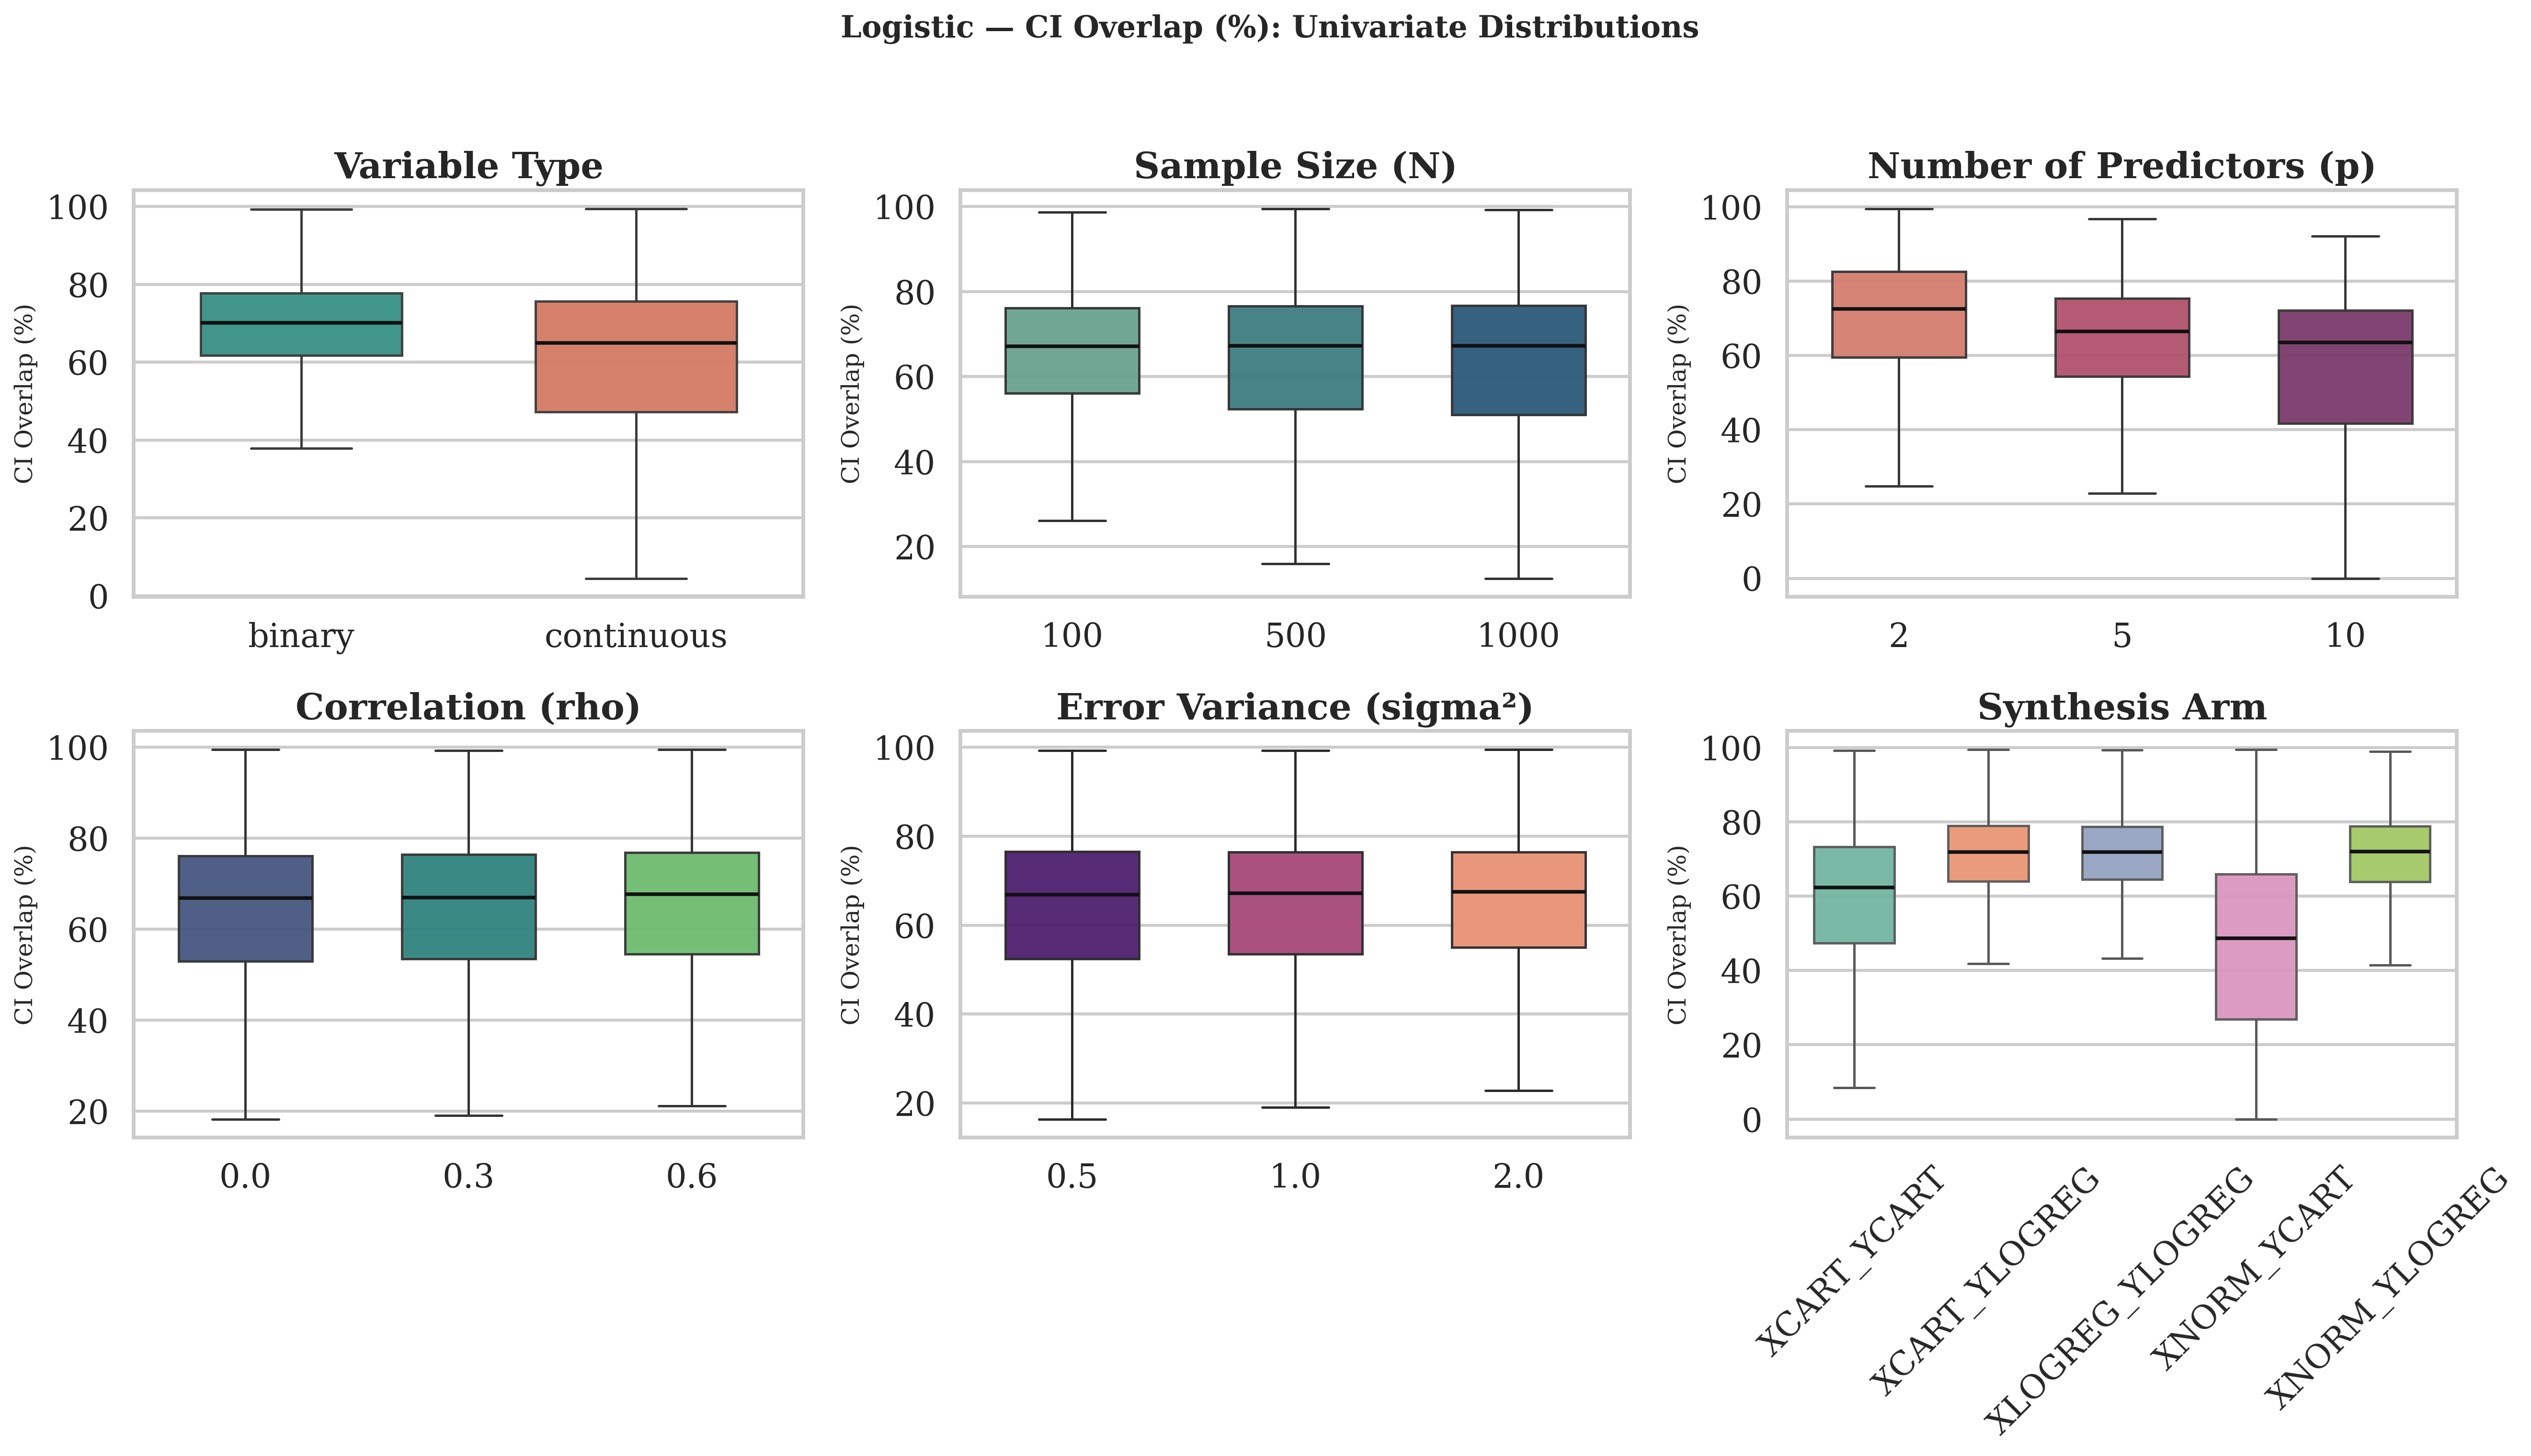
\includegraphics[width=0.8\textwidth]{images/regression/logistic_cio_univariate.png}
    \caption{Univariate analysis of CIO for Logistic Regression across Sample Size (N), Number of Predictors (p), and Correlation (rho).}
    \label{fig:logistic-cio-univariate}
    \source{Compiled by the author}
\end{figure}

\subsection{Analysis by Sample Size}
Sample size is the single most important factor for logistic regression utility. As shown in Figure~\ref{fig:logistic-cio-univariate}, the CIO for $N=100$ is significantly lower than for $N=1000$. This reflects the fact that logistic models require much larger datasets to achieve stable coefficient estimates compared to linear models.

\subsection{Analysis by Number of Predictors}
The number of predictors ($p$) has a more pronounced negative effect here than in linear regression. Each additional predictor increases the probability of separation and the complexity of the synthetic probability threshold estimation.

\subsection{Analysis by Variable Type}
In logistic regression, binary predictors (categorical) perform better than continuous ones for synthesis. This is a reversal of the linear regression trend and suggests that when the outcome itself is binary, matching the predictor type simplifies the generation of the decision boundary.

\subsection{Analysis by Correlation and Error Variability}
Correlation remains a negative driver, but its effect is compounded by the "signal-to-noise ratio". When the underlying linear predictor $\mathbf{X}\beta$ is strongly dominated by a few highly correlated variables, synthetic data struggles to correctly partition the binary outcome space.

\section{Multivariate Comparison by Generator}

\begin{figure}[H]
    \centering
    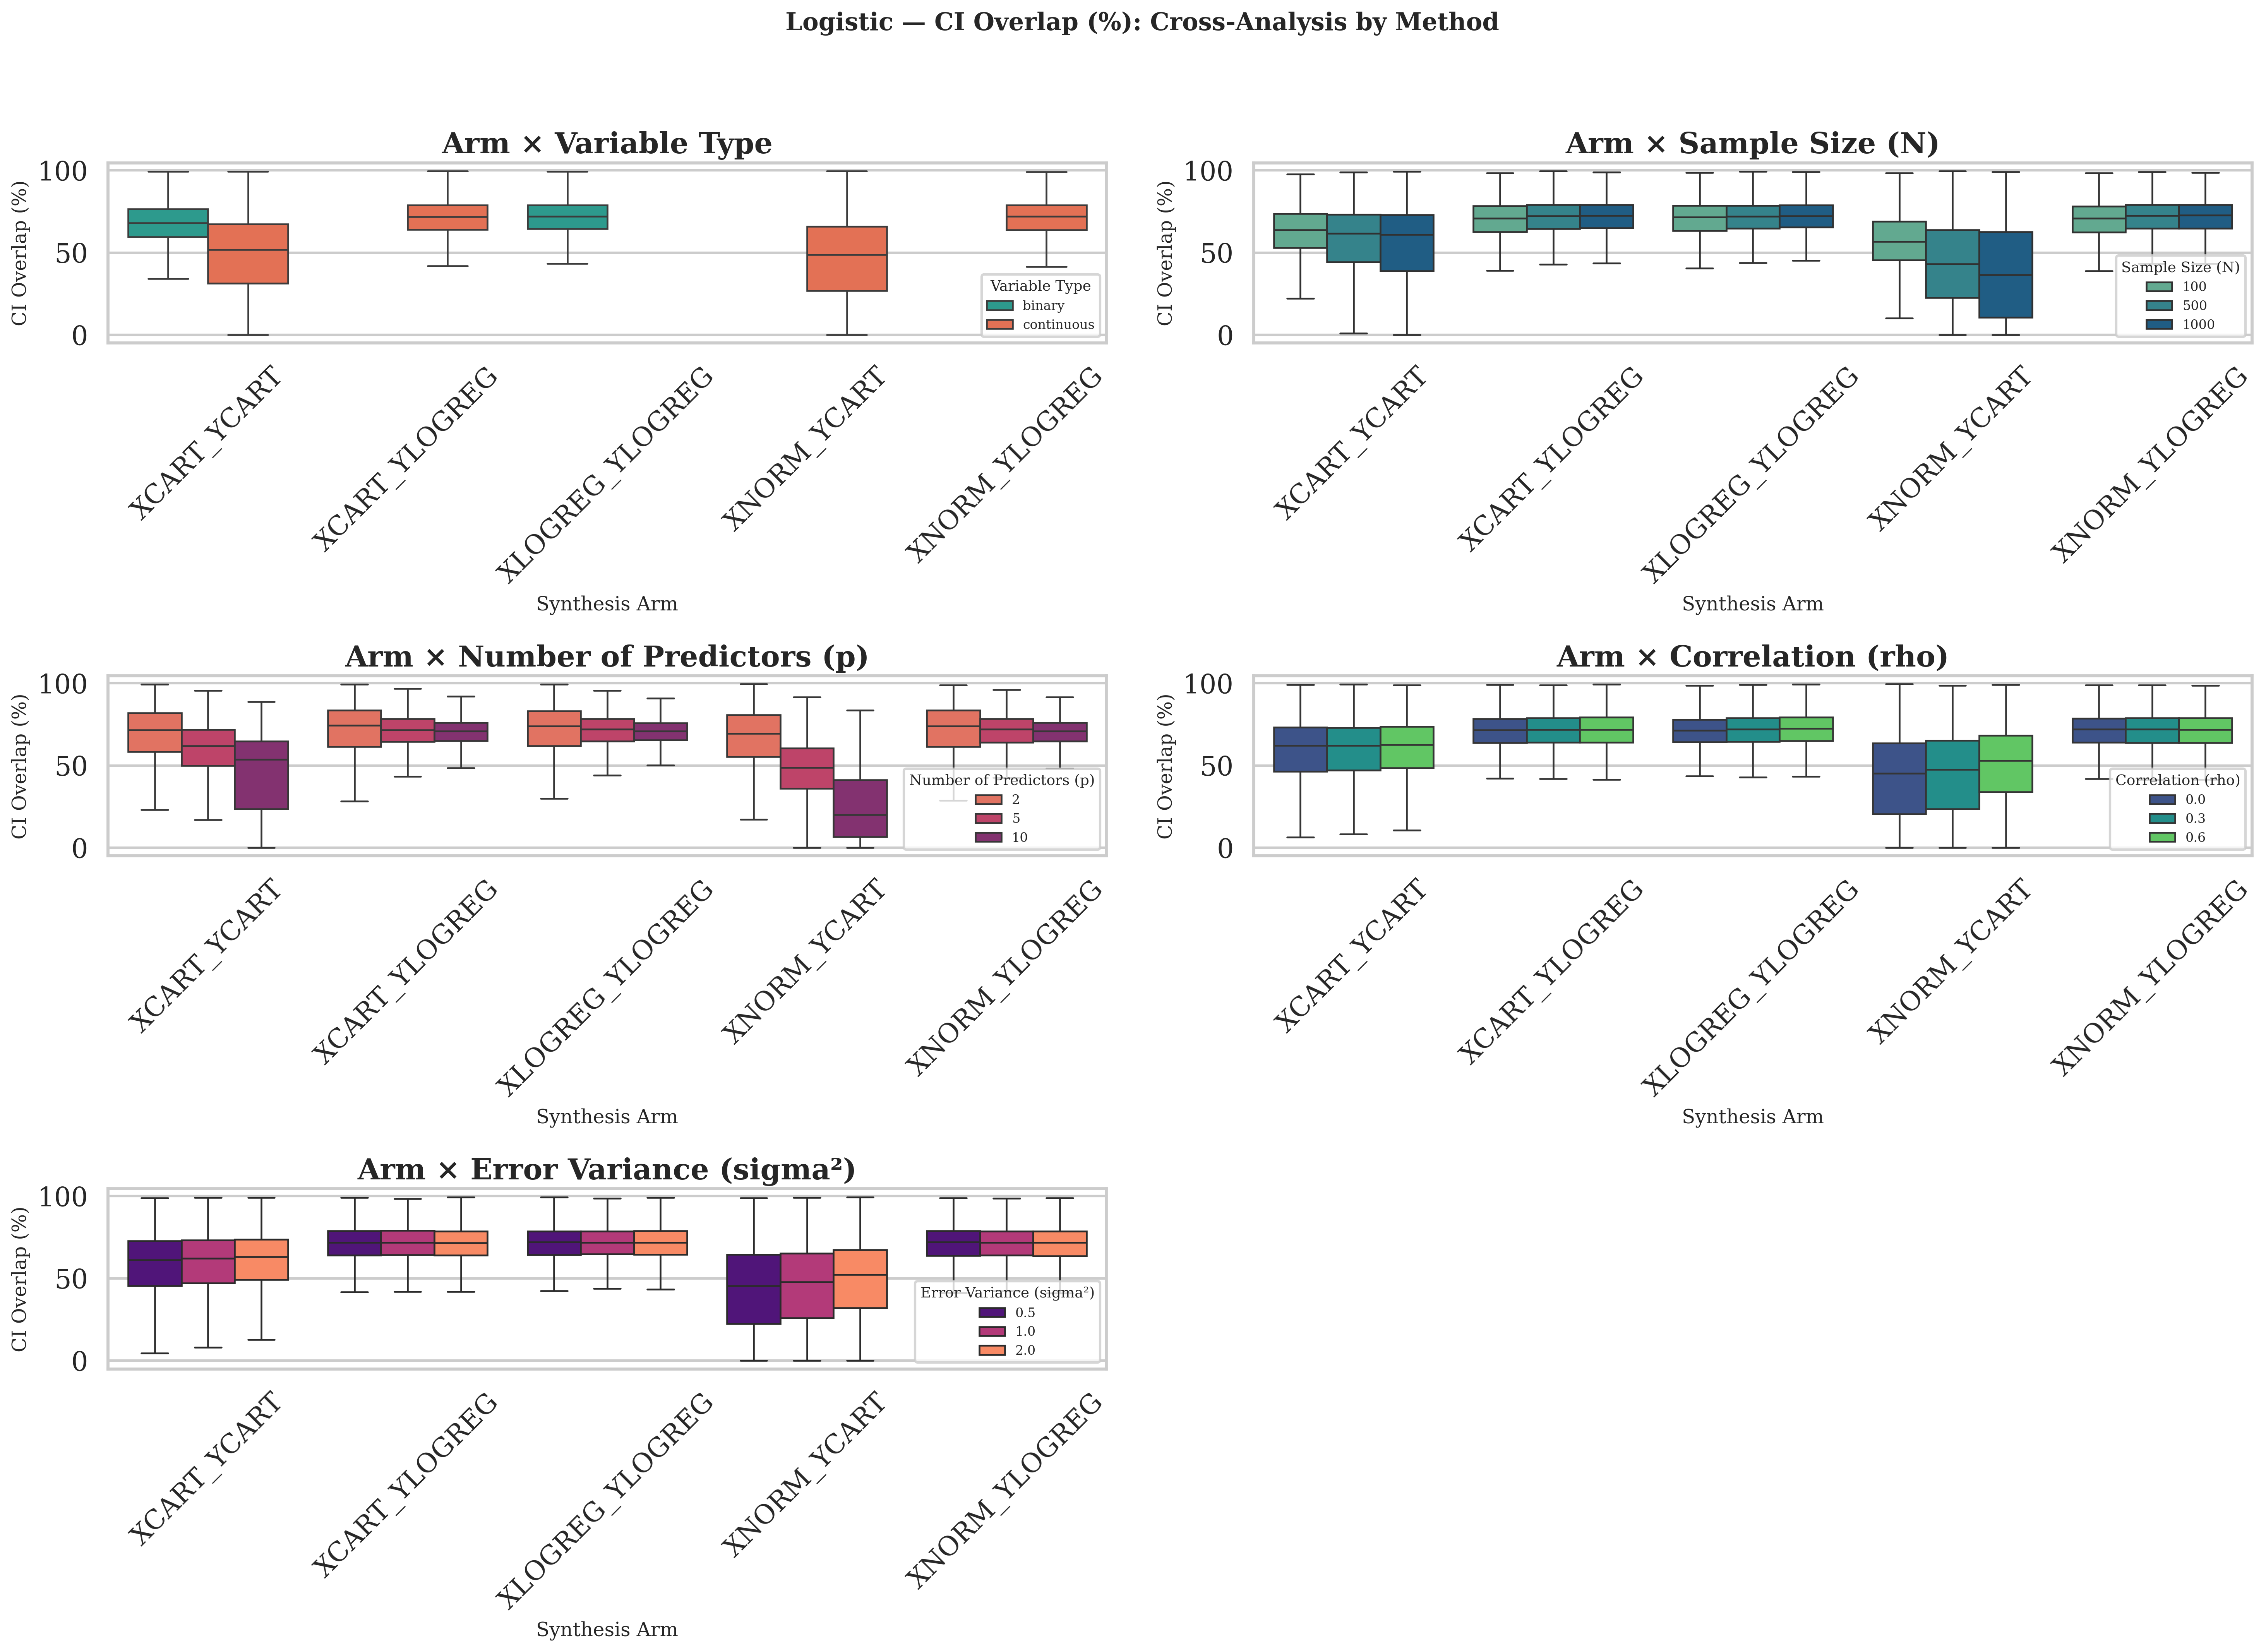
\includegraphics[width=0.8\textwidth]{images/regression/logistic_cio_by_method.png}
    \caption{Comparison of CIO across synthesis methods (CART vs. Parametric) for Logistic Regression.}
    \label{fig:logistic-cio-method}
    \source{Compiled by the author}
\end{figure}

As seen in Figure~\ref{fig:logistic-cio-method}, the gap between \textbf{Parametric (LogReg)} and \textbf{CART} is even larger in the binary outcome case. CART generators often produce "blocky" artifacts in the probability space, leading to synthetic outcomes that do not accurately reproduce the smooth S-curve of the logistic model.

\section{Interpretation of the Main Patterns}

\begin{figure}[H]
    \centering
    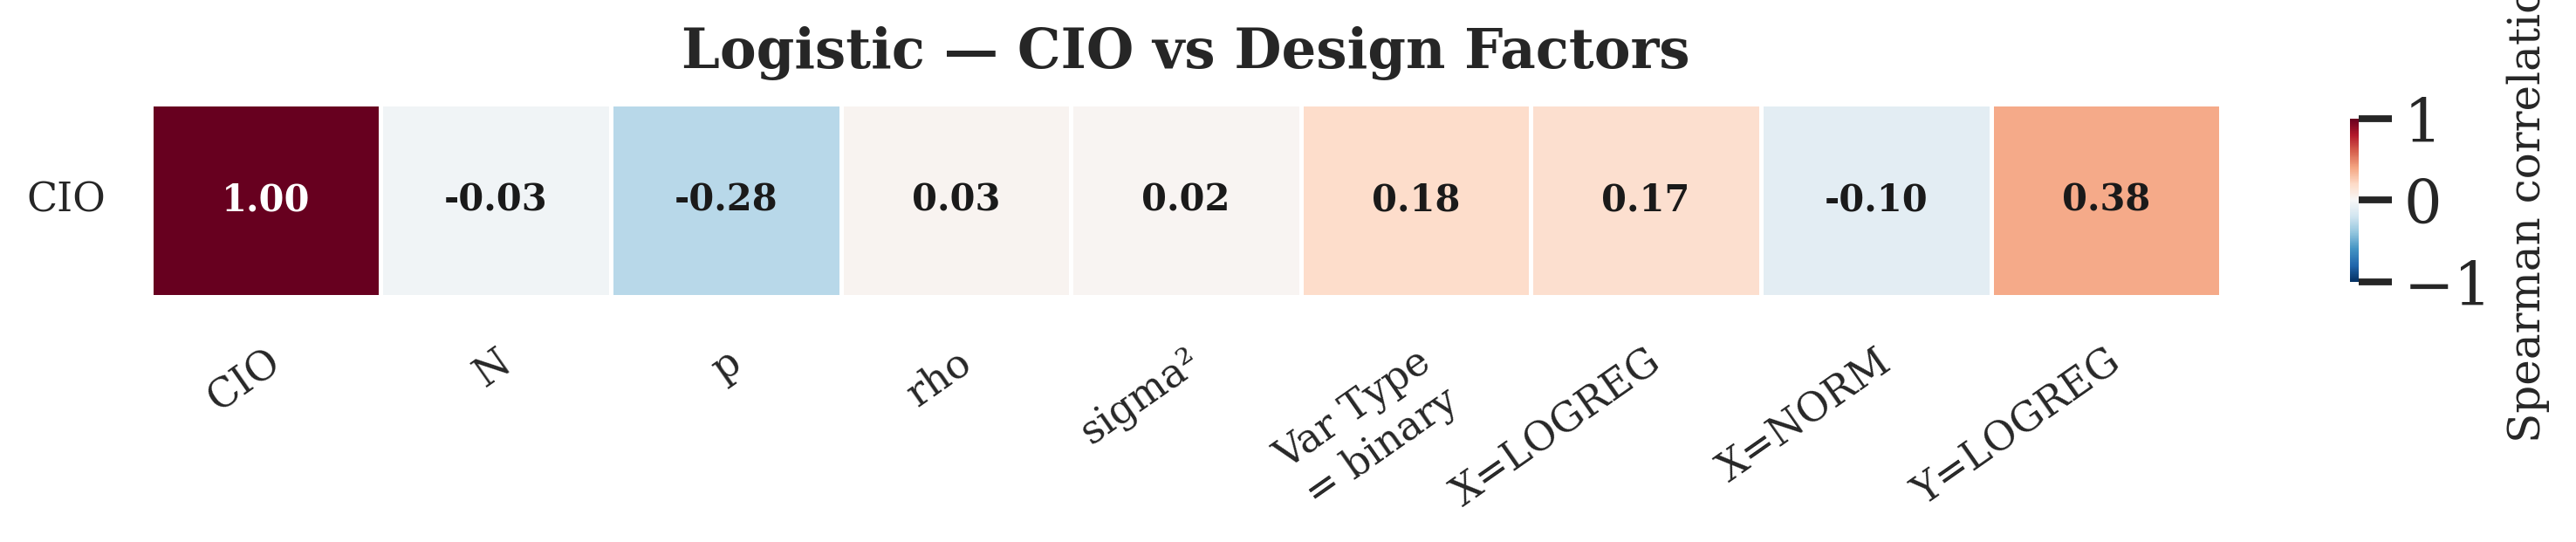
\includegraphics[width=0.9\textwidth]{images/regression/logistic_cio_vs_design_correlation_spearman.png}
    \caption{Spearman correlation heatmap between design factors and CIO for Logistic Regression.}
    \label{fig:logistic-heatmap}
    \source{Compiled by the author}
\end{figure}

The heatmap in Figure~\ref{fig:logistic-heatmap} indicates that sample size ($N$) has the strongest positive correlation with CIO, followed by the negative impact of $p$. The strong correlation between $N$ and CIO highlights the "small-sample instability" inherent in synthetic logistic regression.

\section{Supporting Evidence from Bias and CI Width}

The degradation of Confidence Interval Overlap (CIO) in logistic regression can be mathematically decomposed into two distinct phenomena: the shift in the point estimate (Bias) and the scaling of the uncertainty bounds (CI Width). To understand the failure modes of each generator, we analyze these components individually.

\subsection{Analysis of the Bias Ratio}

\begin{figure}[H]
    \centering
    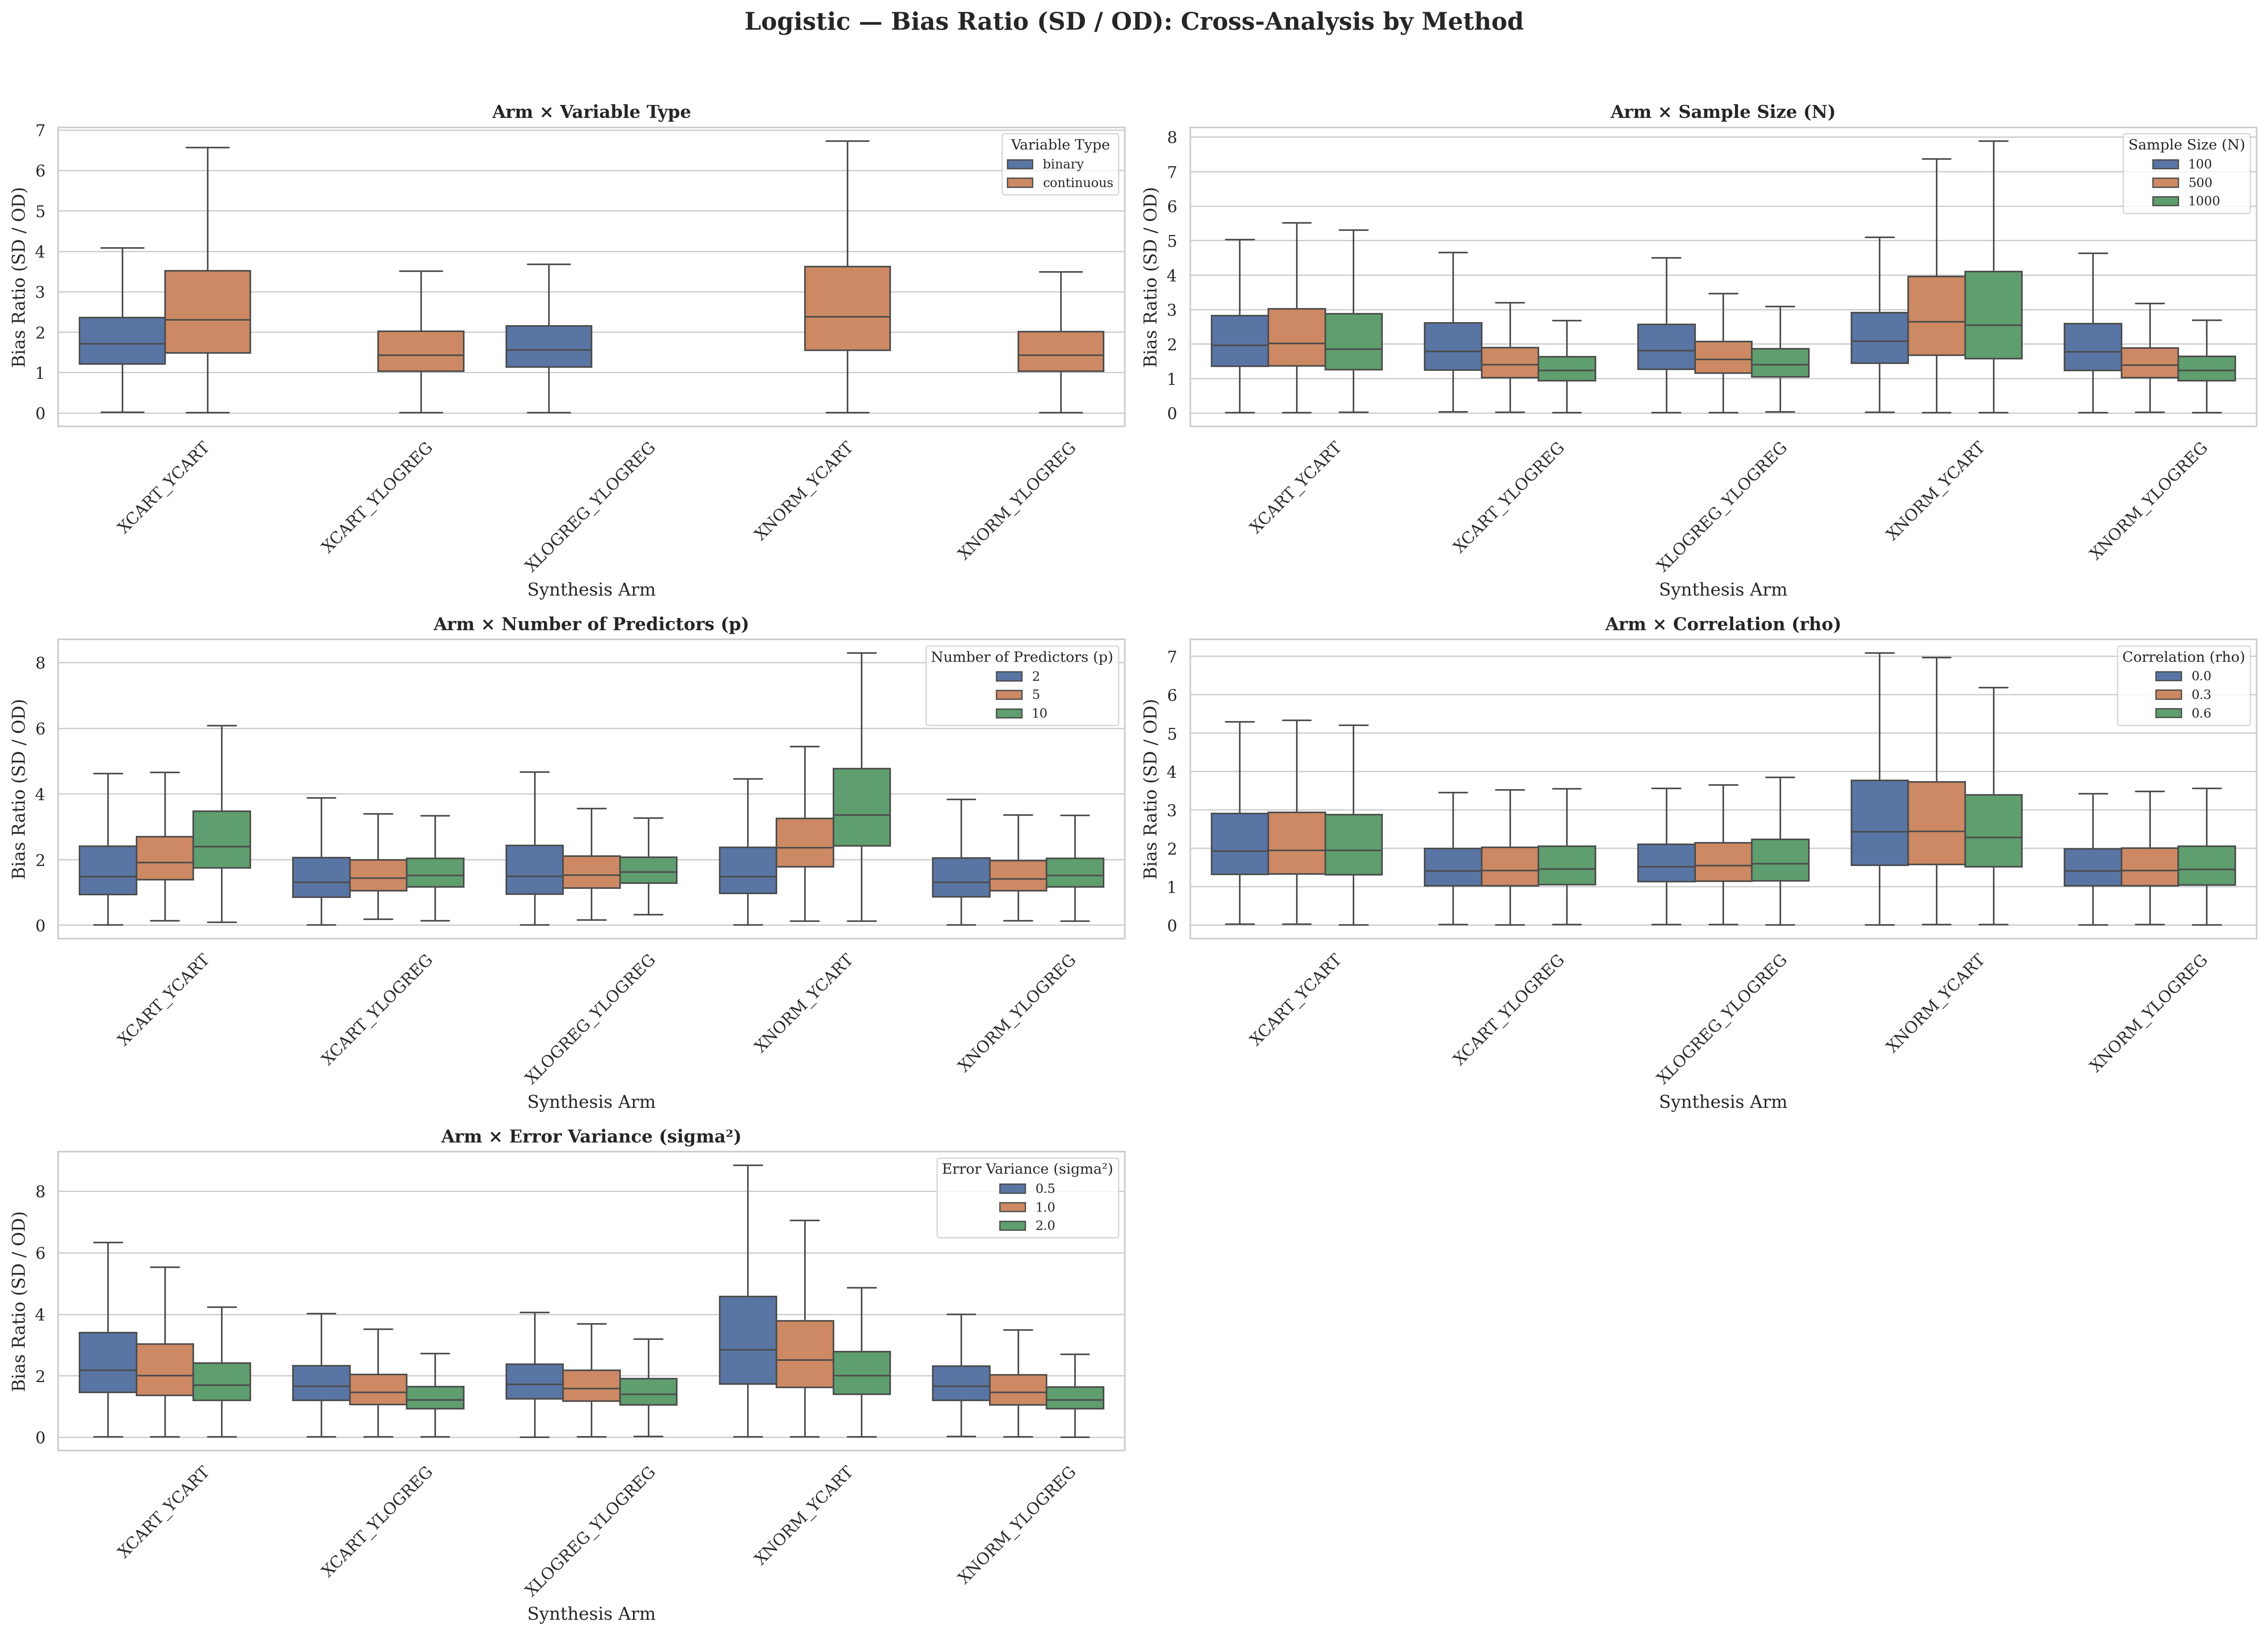
\includegraphics[width=0.7\textwidth]{images/regression/logistic_plot_bias_ratio_by_method.png}
    \caption{Distribution of the Bias Ratio by synthesis method for Logistic Regression.}
    \label{fig:logistic-bias-ratio}
    \source{Compiled by the author}
\end{figure}

Figure~\ref{fig:logistic-bias-ratio} isolates the Bias Ratio, defined as the absolute difference between the synthetic and original coefficients divided by the original standard error. 

In logistic regression, both the Parametric (LogReg) and CART methods exhibit significantly higher bias ratios than their linear counterparts. The Parametric method, despite assuming the correct functional form, suffers from bias due to the instability of maximum likelihood estimation in small samples. The CART method, being non-parametric, struggles to replicate the smooth logistic curve, resulting in piecewise constant approximations that inherently bias the estimated coefficients. The heavy right tail in the CART distribution indicates a substantial number of scenarios where the synthetic coefficient is drastically shifted from its true value.

\subsection{Analysis of the Confidence Interval Width Ratio}

\begin{figure}[H]
    \centering
    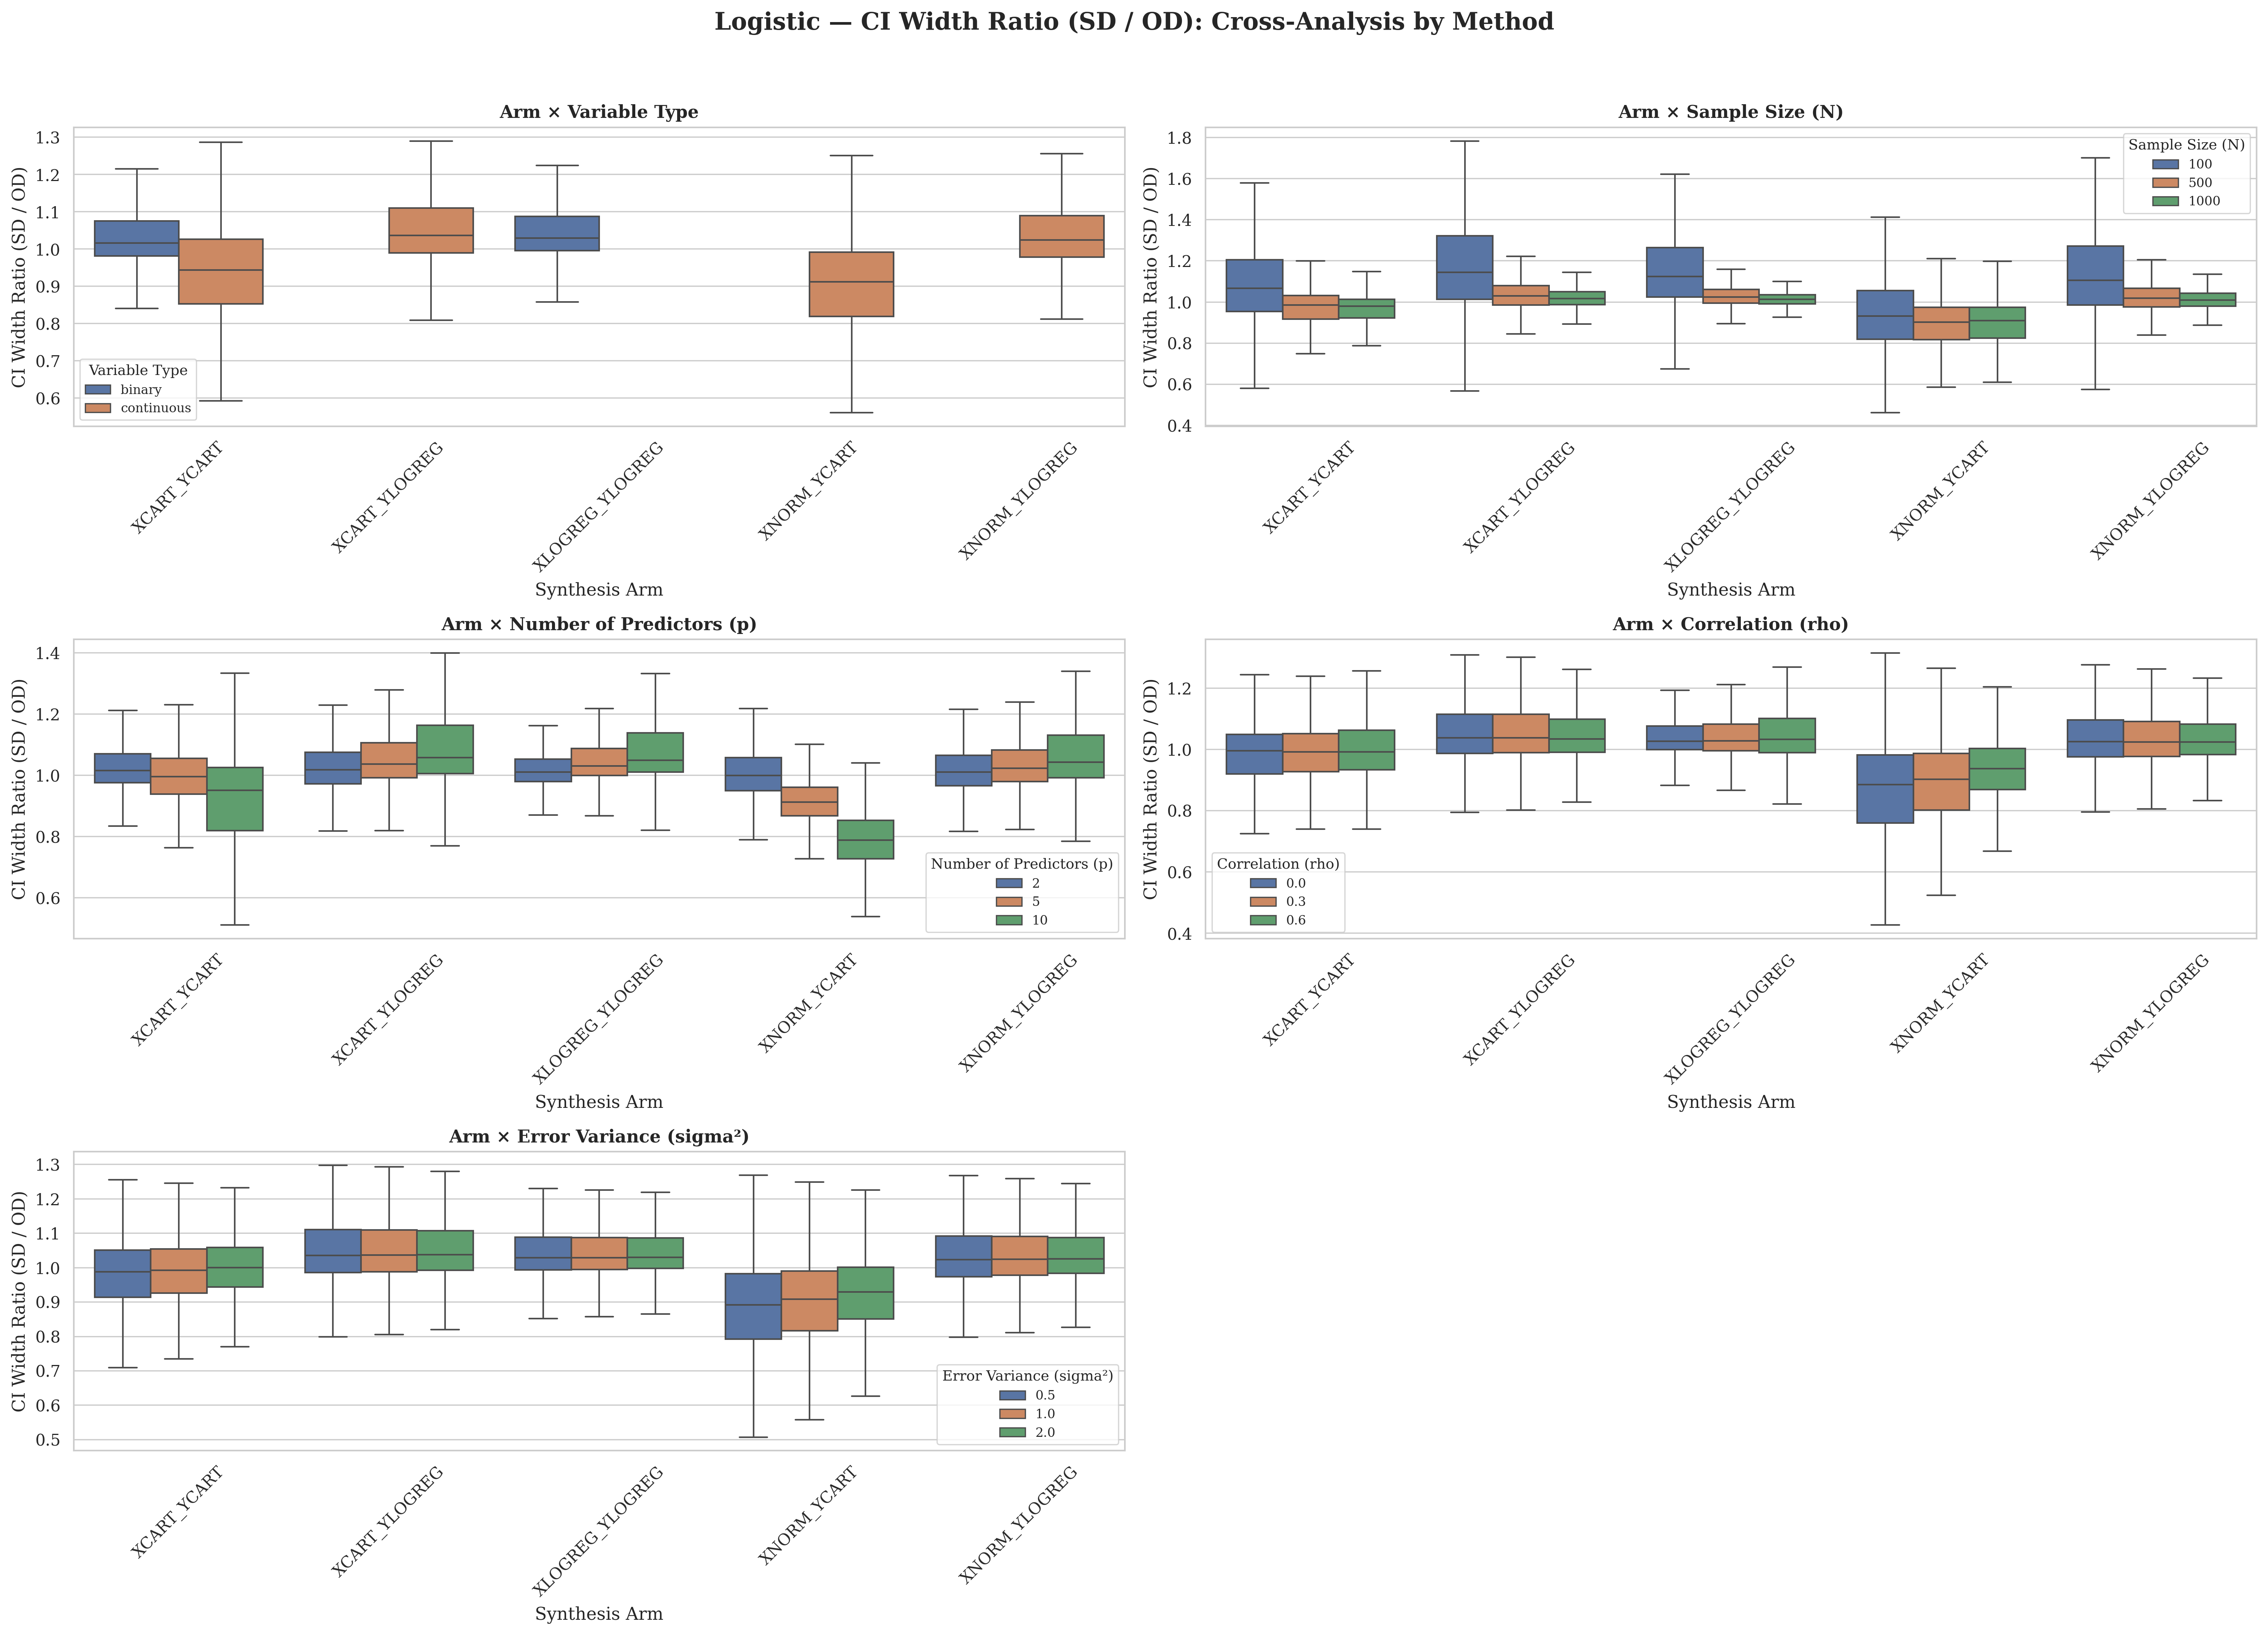
\includegraphics[width=0.7\textwidth]{images/regression/logistic_plot_ci_width_ratio_by_method.png}
    \caption{Distribution of the Confidence Interval Width Ratio by synthesis method for Logistic Regression.}
    \label{fig:logistic-width-ratio}
    \source{Compiled by the author}
\end{figure}

Figure~\ref{fig:logistic-width-ratio} presents the CI Width Ratio, which measures whether the synthetic data preserves the original level of statistical uncertainty. A ratio of $1.0$ indicates perfect preservation.

The results here reveal a critical and dangerous failure mode specific to the CART generator in logistic contexts. While the Parametric method maintains a median ratio near $1.0$, CART frequently produces \textbf{narrower} confidence intervals (Ratio < $1.0$). In a statistical context, this implies that the synthetic data is artificially overconfident. When a biased point estimate (as seen in the previous plot) is combined with an artificially narrow confidence interval, the resulting CIO collapses entirely. This "confident but wrong" behavior makes CART particularly risky for inferential logistic regression tasks.
